\begin{infocard}{Triángulo isósceles}
    % \begin{minipage}{0.25\textwidth}
    \begin{figure}[H]
        \centering
        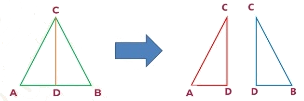
\includegraphics[width=0.9\linewidth]{../images/triangulo_isosceles.png}
    \end{figure}
    % \end{minipage}%
    % \begin{minipage}{0.7\textwidth}
    Si $\triangle ABC$ es un triángulo isósceles, entonces \[\triangle ADC \cong \triangle DBC\]
    % \end{minipage}
    % \newcommand{\pythagwidth}{3cm}
    % \newcommand{\pythagheight}{2cm}

    % \begin{tikzpicture}

    %     \coordinate [label={below right:$A$}] (A) at (0, 0);
    %     \coordinate [label={above right:$B$}] (B) at (0, \pythagheight);
    %     \coordinate [label={below left:$C$}] (C) at (-\pythagwidth, 0);

    %     \coordinate (D1) at (-\pythagheight, \pythagheight + \pythagwidth);
    %     \coordinate (D2) at (-\pythagheight - \pythagwidth, \pythagwidth);

    %     \draw [very thick] (A) -- (C) -- (B) -- (A);

    %     \newcommand{\ranglesize}{0.3cm}
    %     \draw (A) -- ++ (0, \ranglesize) -- ++ (-\ranglesize, 0) -- ++ (0, -\ranglesize);

    %     \draw [dashed] (A) -- node [below] {$b$} ++ (-\pythagwidth, 0)
    %     -- node [right] {$b$} ++ (0, -\pythagwidth)
    %     -- node [above] {$b$} ++ (\pythagwidth, 0)
    %     -- node [left] {$b$} ++ (0, \pythagwidth);

    %     \draw [dashed] (A) -- node [right] {$c$} ++ (0, \pythagheight)
    %     -- node [below] {$c$} ++ (\pythagheight, 0)
    %     -- node [left] {$c$} ++ (0, -\pythagheight)
    %     -- node [above] {$c$} ++ (-\pythagheight, 0);

    %     \draw [dashed] (C) -- node [above left] {$a$} (B)
    %     -- node [below left] {$a$} (D1)
    %     -- node [below right] {$a$} (D2)
    %     -- node [above right] {$a$} (C);

    % \end{tikzpicture}
\end{infocard}